% ─────────────────────────────────────────────────────────────────────────────
\section{Literature Review}
\label{sec:litreview}
% ─────────────────────────────────────────────────────────────────────────────

The 22 selected papers are organised into five thematic subsections, each addressing a
distinct dimension of multi-agent clinical AI design.
Section~\ref{subsec:foundational} reviews the foundational multi-agent frameworks that
established the core architectural vocabulary.
Section~\ref{subsec:coordination} examines agent coordination architectures and
workflow orchestration mechanisms.
Section~\ref{subsec:deliberation} addresses inter-agent deliberation, debate, and
conflict resolution.
Section~\ref{subsec:domain} surveys domain-specific clinical workflow deployments that
provide empirical validation of multi-agent approaches.
Section~\ref{subsec:safety} reviews the limited but critical literature on safety,
robustness, and evaluation of clinical multi-agent systems.

% ─────────────────────────────────────────────────────────────────────────────
\subsection{Foundational Multi-Agent Frameworks for Clinical AI}
\label{subsec:foundational}
% ─────────────────────────────────────────────────────────────────────────────

This subsection reviews the earliest and most foundational multi-agent frameworks applied
to clinical AI tasks.  These four works established the core architectural concepts ---
role-playing agents, iterative discussion loops, consensus-based synthesis, and
supervisory oversight --- upon which all subsequent research in this chapter is
built.  The progression from MedAgents'
benchmark-only evaluation through to the MAC Framework's publication in a high-impact
clinical journal illustrates the rapid maturation of the field between 2024 and
2025.  Table~\ref{tab:tracker_foundational} provides an overview of the four papers
reviewed in this subsection before the detailed discussion that follows.

\begin{table}[ht]
\centering
\caption{Literature Tracker: Foundational Multi-Agent Frameworks}
\label{tab:tracker_foundational}
\begin{adjustbox}{max width=\textwidth}
\begin{tabular}{p{2.2cm} p{2.5cm} p{2.2cm} p{3.2cm} p{3.0cm}}
\toprule
\textbf{Paper} & \textbf{Architecture Type} & \textbf{Evaluation Scope} & \textbf{Key Finding} & \textbf{Thesis Relevance} \\
\midrule
MedAgents~\cite{Tang2024MedAgents}
  & Role-play + iterative discussion
  & 9 benchmarks (zero-shot)
  & 77\% errors from knowledge gaps
  & Foundational MAS paradigm; knowledge-pooling justification \\[3pt]
openCHA~\cite{Abbasian2024openCHA}
  & Three-layer orchestrator with external sources
  & 2 demos + 4 use cases
  & 92\% ChatDiet effectiveness; outperformed GPT-4
  & Task Planner + Executor architecture precedent \\[3pt]
AI Hospital~\cite{Fan2024AIHospital}
  & 4-role simulation with Chief Physician
  & MVME benchmark; multi-turn
  & Dispute resolution structurally necessary
  & Proves conflict resolution is required \\[3pt]
MAC~\cite{MAC2025npj}
  & MDT with Supervisor
  & 302 rare disease cases
  & 4 doctors + supervisor optimal; beats Self-Consistency
  & Structured discussion more efficient than sampling \\
\bottomrule
\end{tabular}
\end{adjustbox}
\end{table}

The foundational work in this space is MedAgents, introduced by
Tang~et~al.~\cite{Tang2024MedAgents} at ACL 2024 as the first systematic training-free
multi-agent framework for medical reasoning.  The framework operates through a five-step
pipeline: domain expert agents are assembled through role-assignment prompting; each
agent independently analyses the clinical query; individual analyses are synthesised
into a collective report; agents engage in iterative discussion rounds until consensus
is reached; and a final decision is produced.  Evaluated across nine medical benchmarks
--- including MedQA, MedMCQA, PubMedQA, and six MMLU medical subtasks --- MedAgents
outperformed all baselines in a zero-shot setting, including domain-specific fine-tuned
models such as MedAlpaca-7B and BioMedGPT-10B~\cite{Tang2024MedAgents}.  The iterative
discussion phase was identified as the highest-value component in ablation experiments.
Most importantly, an error analysis of 300 cases established that 77\% of LLM medical
errors result from domain knowledge gaps rather than reasoning failures, providing the
clearest empirical justification for the multi-agent knowledge-pooling approach over
single-model alternatives.  The work has several limitations: evaluation is confined to
multiple-choice question-answering benchmarks with no integration of clinical workflows
or real patient data; all agents share the same underlying LLM, meaning correlated
knowledge gaps cannot be resolved through discussion; and the fixed discussion rounds
have no adaptive stopping criterion~\cite{Lu2024TriageAgent}.  Nevertheless, MedAgents
is the foundational work from which the entire subsequent literature draws its core
architectural vocabulary --- the role-playing agent, the iterative discussion loop, and
the consensus-based synthesis pattern.

While MedAgents established the multi-agent discussion paradigm, it lacked integration
with real-time clinical data sources and external tools.
Abbasian~et~al.~\cite{Abbasian2024openCHA} addressed this gap with openCHA, an
open-source LLM-powered framework published in JAMIA Open 2024 that introduces a
three-layer architecture: an Interface layer for multimodal input, an Orchestrator for
multi-step reasoning and delegation, and a set of External Sources for real-time clinical
data access.  The Orchestrator comprises five sub-components: a Task Planner
implementing Tree of Thought prompting to generate and evaluate candidate action
strategies, a Task Executor, a Data Pipe for intermediate result storage, a Promptist
for prompt construction, and a dedicated Response
Generator~\cite{Abbasian2024openCHA}.  The framework was validated through two live
demonstrations and four real-world use cases, demonstrating consistent outperformance of
GPT-4 and ChatGPT on clinical tasks including dietary guidance (92\% effectiveness in
the ChatDiet use case), diabetes management, and mental health chatbot safety evaluation.
The bidirectional communication loop between the Task Planner and Task Executor ---
which allows intermediate findings from execution to inform subsequent planning --- is an
architectural innovation that models the genuine iterative problem-solving observed in
expert clinical reasoning~\cite{Shang2025DynamiCare}.  The primary limitations are the
absence of parallel agent execution and the lack of any inter-agent negotiation or
conflict-handling mechanism~\cite{Fan2024AIHospital}.

The question of what happens when agents within a multi-agent clinical system disagree
was first addressed empirically by Fan~et~al.~\cite{Fan2024AIHospital}, who introduced
AI Hospital as a multi-agent simulation environment modelling a complete clinical episode
through four interacting agent roles: a Doctor agent conducting an iterative medical
consultation, a Patient agent that discloses symptoms progressively, an Examiner agent
executing medical tests, and a Chief Physician agent overseeing the consultation and
participating in dispute resolution.  The Multi-View Medical Evaluation (MVME) benchmark
was introduced alongside the framework~\cite{Fan2024AIHospital}.  The study revealed a
significant finding: in multi-turn interactive diagnostic workflows, all tested LLMs
achieved less than 50\% of the diagnostic accuracy recorded under the single-pass
full-information condition, establishing multi-turn clinical information gathering as a
critical unsolved capability gap.  Furthermore, removing the dispute resolution mechanism
from the multi-doctor configuration caused a statistically significant reduction in
diagnostic accuracy, demonstrating for the first time that structured conflict resolution
is a structurally necessary component of multi-agent clinical
systems~\cite{Wang2025Catfish}.

Building on these foundations, the Multi-Agent Conversation (MAC) framework, published
by Shen~et~al.~\cite{MAC2025npj} in \textit{npj Digital Medicine} --- the
highest-impact journal represented in this review --- brought multi-agent clinical AI to
peer-reviewed clinical publication.  MAC models clinical diagnosis as a structured group
consultation in which multiple Doctor agents conduct iterative discussion rounds of
proposal, critique, and refinement under the supervision of a Supervisor
agent~\cite{MAC2025npj}.  Evaluated on 302 rare disease cases using GPT-4, MAC
outperformed all baselines on both primary and follow-up consultation tasks.  The optimal
configuration --- empirically determined through ablation --- was four Doctor agents plus
one Supervisor, with performance declining for larger team sizes due to redundant
discussion.  Critically, the MAC framework outperformed Self-Consistency despite
Self-Consistency using more total model inference calls, establishing that structured
role-based discussion is a more computationally efficient and more accurate mechanism
than parallel independent sampling~\cite{Chen2025MDTeamGPT}.

% ─────────────────────────────────────────────────────────────────────────────
\subsection{Agent Coordination Architectures and Workflow Orchestration}
\label{subsec:coordination}
% ─────────────────────────────────────────────────────────────────────────────

The foundational frameworks reviewed above established that multi-agent systems
outperform single models on clinical tasks, but they largely employed fixed agent
configurations regardless of task complexity~\cite{Tang2024MedAgents}.  This subsection
examines the second thematic cluster of papers, which make explicit architectural
contributions to the problem of coordinating multiple agents within structured workflows
--- covering adaptive routing, hierarchical escalation, workflow decomposition, the
theoretical limits of component-level optimisation, and dynamic iterative
loops.  Table~\ref{tab:tracker_coordination}
provides an overview before the detailed discussion.

\begin{table}[ht]
\centering
\caption{Literature Tracker: Agent Coordination Architectures}
\label{tab:tracker_coordination}
\begin{adjustbox}{max width=\textwidth}
\begin{tabular}{p{2.2cm} p{2.5cm} p{2.2cm} p{3.2cm} p{3.0cm}}
\toprule
\textbf{Paper} & \textbf{Architecture Type} & \textbf{Evaluation Scope} & \textbf{Key Finding} & \textbf{Thesis Relevance} \\
\midrule
MDAgents~\cite{Kim2024MDAgents}
  & Adaptive complexity routing
  & 10 benchmarks; GPT-4 + Gemini
  & Best on 7/10; $+$4.2\% over fixed
  & Core orchestration precedent \\[3pt]
TAO~\cite{Kim2025TAO}
  & 3-tier safety hierarchy
  & 5 safety benchmarks
  & Reduced harmfulness; outperformed MDAgents on safety
  & Tiered escalation precedent \\[3pt]
Opt.\ Paradox~\cite{Bedi2025OptParadox}
  & Best-of-Breed vs.\ homogeneous
  & 2{,}400 MIMIC-CDM cases
  & Coordination $>$ component quality; 13.87\% hallucination
  & Defines the exact gap this thesis addresses \\[3pt]
Barra et al.~\cite{Barra2025Agentic}
  & 7-agent n8n pipeline; 5 patterns
  & 50 test runs
  & 70--80\% time reduction
  & Direct workflow design precedent \\[3pt]
DynamiCare~\cite{Shang2025DynamiCare}
  & Dynamic multi-round with Patient Agent
  & MIMIC-Patient benchmark
  & Dynamic outperforms single-pass
  & First iterative adaptive loop model \\
\bottomrule
\end{tabular}
\end{adjustbox}
\end{table}

The first major step toward adaptive coordination was MDAgents, proposed by
Kim~et~al.~\cite{Kim2024MDAgents} at NeurIPS 2024, which introduced the first fully
adaptive multi-agent framework for medical decision-making.  Rather than deploying a
fixed agent configuration for all inputs, MDAgents classifies each query as low,
moderate, or high complexity, and recruits a solo agent, a group of collaborating agents
with a Moderator, or a full multi-disciplinary team
accordingly~\cite{Kim2024MDAgents}.  Evaluated across ten medical benchmark datasets
using GPT-4 and Gemini as backbones, MDAgents achieved best performance on seven of the
ten benchmarks.  The adaptive configuration outperformed both the fixed solo and fixed
group baselines by up to 4.2\% ($p < 0.05$), and incorporating a Moderator agent with
retrieval access improved group-level accuracy by a further 11.8\%.  The framework's
processing latency ranged from 14.7~seconds for low-complexity queries to 226~seconds
for high-complexity multi-team deliberations~\cite{Kim2024MDAgents}.

While MDAgents focused on complexity-based routing for accuracy, the same research group
extended the paradigm to address clinical safety with Tiered Agentic Oversight (TAO),
proposed by Kim~et~al.~\cite{Kim2025TAO} at ICML 2025.  TAO maps the clinical
supervision hierarchy onto a three-tier agent architecture: Tier~1 handles routine
low-risk queries through generalist agents, Tier~2 routes moderate-complexity cases to
specialist agents, and Tier~3 manages high-risk decisions requiring the highest level of
oversight~\cite{Kim2025TAO}.  An Agent Recruiter assigns incoming tasks to the initial
tier, while an Agent Router monitors execution and triggers tier escalation when a
lower-tier agent signals uncertainty.  Compared to MDAgents~\cite{Kim2024MDAgents}, TAO
outperformed specifically on safety-focused benchmarks, demonstrating that an
architecture designed around safety objectives yields measurably superior safety
outcomes~\cite{Chen2025MedSentry}.

The most theoretically significant contribution to the coordination problem came from
Bedi~et~al.~\cite{Bedi2025OptParadox}, who empirically identified the Optimisation
Paradox in clinical AI multi-agent systems.  Using 2{,}400 real patient cases from the
MIMIC-CDM dataset across four abdominal pathologies, the authors compared a single
end-to-end agent, a homogeneous multi-agent system optimised for coordinated
interaction, and a Best-of-Breed heterogeneous system that selected the
highest-performing individual agent for each of four workflow
stages~\cite{Bedi2025OptParadox}.  The Best-of-Breed system achieved only 67.7\%
diagnostic accuracy and a clinically unacceptable test result hallucination rate of
13.87\%.  The homogeneous system, built from less capable but coordination-optimised
components, substantially outperformed it.  The Best-of-Breed system maintained 85.5\%
information accuracy while failing at diagnosis, revealing a stark disconnect between
accurate information retrieval and accurate clinical synthesis across agent
boundaries~\cite{Bedi2025OptParadox}.  This finding establishes coordination
architecture as a primary design parameter that cannot be recovered by optimising
individual agents in isolation, and it represents perhaps the most directly relevant
theoretical contribution to this thesis.  Figure~\ref{fig:opt_paradox} illustrates the
multi-agent system architecture and an example clinical workflow from this study.

\begin{figure}[ht]
\centering
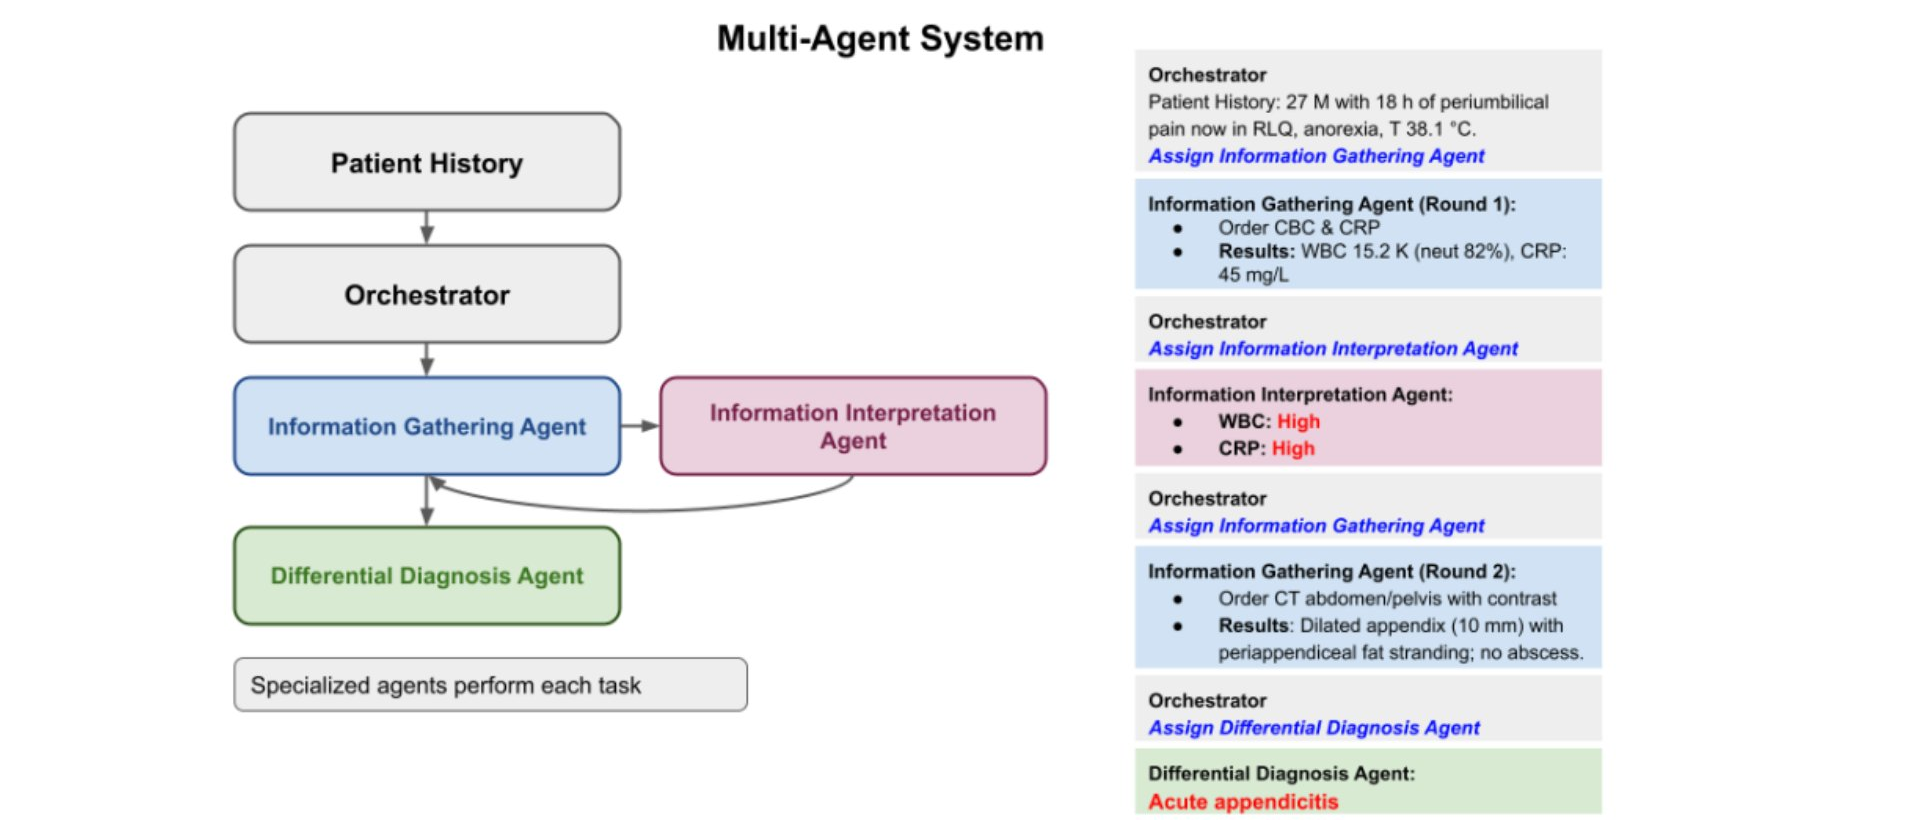
\includegraphics[width=0.95\textwidth]{images/opt_paradox_fig3}
\caption[Multi-agent system architecture from the Optimisation Paradox study]{Multi-agent system (left) and example workflow (right) from Bedi~et~al.~\cite{Bedi2025OptParadox}, where an orchestrator coordinates specialised agents for information gathering, interpretation, and differential diagnosis, demonstrated with an acute appendicitis case.  The study showed that this coordinated homogeneous system substantially outperformed a Best-of-Breed system assembled from individually superior components --- establishing coordination architecture as the primary design variable.}
\label{fig:opt_paradox}
\end{figure}

Complementing these theoretical insights with practical implementation,
Barra~et~al.~\cite{Barra2025Agentic} provided the most detailed automation workflow for
healthcare in the reviewed literature, published in \textit{Advances in Simulation} in
2025.  Using the n8n no-code automation platform, the authors constructed a seven-agent
pipeline incorporating five core workflow design patterns: task decomposition, prompt
chaining, parallelisation, retrieval-augmented generation, and iterative
refinement~\cite{Barra2025Agentic}.  A Reviewer Agent evaluates the complete output
against INACSL and ASPiH standards before an Editor Agent formats the final deliverable.
Across 50 test runs, the pipeline produced complete, standards-compliant simulation
scenarios in an average of 4.5~minutes, representing a 70--80\% reduction in development
time relative to manual authoring~\cite{Barra2025Agentic}.  The
decompose--chain--parallelise--refine pattern and the Reviewer--Editor quality-control
loop established by this work are directly applicable as design precedents for the
automation workflow developed in this thesis.

Finally, Shang~et~al.~\cite{Shang2025DynamiCare} introduced DynamiCare, the first
framework to model clinical diagnosis explicitly as a dynamic, multi-round interactive
process in which the agent team does not receive complete case information upfront but
must iteratively elicit findings through structured queries to a Patient Agent
System~\cite{Shang2025DynamiCare}.  This design mirrors the actual workflow of clinical
consultations, where physicians progressively gather information through history-taking,
physical examination, and investigation ordering~\cite{Fan2024AIHospital}.  The authors
introduced MIMIC-Patient, a new structured dataset derived from MIMIC-III EHR records
constituting the first benchmark specifically designed for dynamic agent-based clinical
decision-making~\cite{Shang2025DynamiCare}.

% ─────────────────────────────────────────────────────────────────────────────
\subsection{Inter-Agent Deliberation, Debate, and Conflict Resolution}
\label{subsec:deliberation}
% ─────────────────────────────────────────────────────────────────────────────

The coordination architectures reviewed above determine how agents are assembled and
routed, but a distinct and equally critical question is what happens when agents within a
system disagree.  This subsection examines a rapidly growing body
of research addressing inter-agent conflict through structured debate, adversarial
dissent injection, and cognitive bias mitigation --- collectively establishing conflict
resolution as a structural necessity for clinical multi-agent systems rather than an
optional
enhancement.
Table~\ref{tab:tracker_deliberation} provides an overview before the detailed
discussion.

\begin{table}[ht]
\centering
\caption{Literature Tracker: Inter-Agent Deliberation and Conflict Resolution}
\label{tab:tracker_deliberation}
\begin{adjustbox}{max width=\textwidth}
\begin{tabular}{p{2.2cm} p{2.5cm} p{2.2cm} p{3.2cm} p{3.0cm}}
\toprule
\textbf{Paper} & \textbf{Architecture Type} & \textbf{Evaluation Scope} & \textbf{Key Finding} & \textbf{Thesis Relevance} \\
\midrule
MDTeamGPT~\cite{Chen2025MDTeamGPT}
  & 4-phase MDT with self-evolution
  & MedQA + MedMCQA; GPT-4
  & Debate $>$ consensus; heterogeneous views drive quality
  & Debate workflow design precedent \\[3pt]
Layered Debate~\cite{Zhao2025LayeredDebate}
  & 3-layer debate with Judge Agent
  & Similar-disease disambiguation
  & Layer~2 adversarial exchange is highest-value component
  & Judge agent precedent \\[3pt]
Catfish Agent~\cite{Wang2025Catfish}
  & Dissent injection agent
  & 12 benchmarks (9 QA + 3 VQA)
  & Silent agreement = systematic failure; Catfish beats GPT-4o
  & Complexity-aware dissent precedent \\[3pt]
Ke et al.~\cite{Ke2024CognitiveBias}
  & 3-role bias mitigation framework
  & 10 clinical vignettes
  & MAS reduces cognitive biases; safety intervention
  & Critical evaluator agent precedent \\
\bottomrule
\end{tabular}
\end{adjustbox}
\end{table}

The earliest work to formalise multi-agent debate for clinical AI is MDTeamGPT, proposed
by Chen~et~al.~\cite{Chen2025MDTeamGPT} at Nanjing University in 2025.  MDTeamGPT
simulates a multi-disciplinary team (MDT) consultation through a four-phase workflow:
role assignment, independent analysis, structured debate, and
synthesis~\cite{Chen2025MDTeamGPT}.  Evaluated on MedQA and MedMCQA using GPT-4,
MDTeamGPT outperformed all baselines including single-agent, fixed-team, and
non-evolving multi-agent configurations.  The structured debate phase was the
highest-value component.  A critical finding is that performance was highest when agents
began the debate with heterogeneous initial diagnoses, establishing diversity of initial
agent views as a measurable quality driver~\cite{Chen2025MDTeamGPT}.

While MDTeamGPT demonstrated the value of debate for general medical reasoning,
Zhao~et~al.~\cite{Zhao2025LayeredDebate} targeted a more specific clinical challenge:
disambiguating diseases with overlapping symptom profiles.  Their Layered Debate
architecture, presented at NAACL 2025, operates through three layers: Layer~1 involves
specialist agents independently generating an initial diagnosis; Layer~2 involves
structured adversarial cross-examination; and Layer~3 involves a dedicated Judge Agent
that reads the full debate transcript and produces a final diagnostic verdict, replacing
the simple majority voting used in earlier
frameworks~\cite{Tang2024MedAgents,MAC2025npj}.  The layered debate architecture
significantly outperformed single-agent, standard multi-agent, and chain-of-thought
baselines on similar-disease disambiguation tasks, and Layer~2 adversarial evidence
exchange was identified as the highest-value
component~\cite{Zhao2025LayeredDebate}.

A deeper structural problem underlying both of these approaches was identified by
Wang~et~al.~\cite{Wang2025Catfish}, who demonstrated that \textit{silent agreement} ---
the systematic tendency of agents in a standard MAS to prematurely converge on a
diagnosis without genuine critical evaluation --- is a pervasive failure mode in clinical
multi-agent frameworks.  The Catfish Agent, proposed as a structural remedy, is a
role-specialised LLM whose sole function is to inject structured dissent into group
deliberation at every round~\cite{Wang2025Catfish}.  Two complementary mechanisms were
introduced: a complexity-aware mechanism that modulates the intensity of dissent based on
the assessed difficulty of the clinical case, and a tone-calibrated mechanism that
balances adversarial critique with collaborative reasoning.  Evaluated across twelve
benchmarks --- nine medical question-answering and three medical visual
question-answering tasks --- the Catfish Agent outperformed all baselines including
GPT-4o and DeepSeek-R1, with the complexity-aware mechanism delivering the largest gains
on ambiguous and diagnostically challenging cases~\cite{Wang2025Catfish}.  Tone
calibration was found to be critical: overly aggressive dissent consistently reduced
performance, while calibrated dissent consistently improved
it~\cite{Wang2025Catfish}.

The connection between agent disagreement and patient safety was made explicit by
Ke~et~al.~\cite{Ke2024CognitiveBias}, who published in JMIR the first controlled
simulation study examining whether multi-agent LLM conversations can reduce the
cognitive biases --- anchoring, availability, and confirmation bias --- that are
well-documented sources of diagnostic error in clinical
medicine~\cite{Ke2024CognitiveBias}.  Ten clinical vignettes were constructed to
reliably elicit each target bias in a single-agent condition, and processed by a
three-role framework comprising a primary decision agent, expert consultant agents, and a
dedicated critical evaluator agent.  Across all ten vignettes, the multi-agent condition
produced significantly fewer cognitive bias occurrences and higher diagnostic accuracy.
The critical evaluator agent was the most effective single component, preventing the
primary agent from persisting with an incorrect initial impression when contradictory
clinical evidence was presented~\cite{Ke2024CognitiveBias}.  This work establishes
multi-agent design as a patient safety intervention rather than merely an efficiency
mechanism~\cite{Kim2025TAO}.
